\begin{frame}{从稳态线性响应到超快 pump--probe}

  \footnotesize
  \setlength{\abovedisplayskip}{1pt}
  \setlength{\belowdisplayskip}{1pt}

  {\centering
    $\text{weak probe}\;\longrightarrow\;\chi(\omega)
      \;\longrightarrow\;T(\omega),R(\omega),A(\omega).$\par}
  {\centering\fontsize{6.5}{7.6}\selectfont\color{gray}
    平稳腔--分子体系可由固定的线性响应 $\chi(\omega)$ 描述。\par}

  \vspace{0.1em}

  \begin{columns}[T,onlytextwidth]
    \begin{column}{0.44\textwidth}
      {\centering
        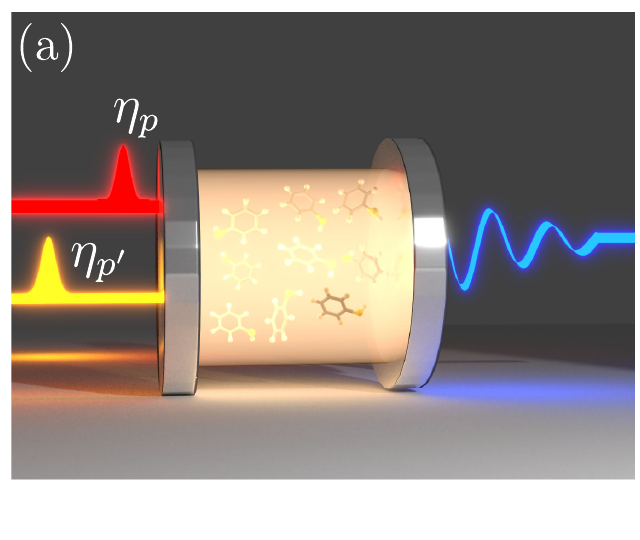
\includegraphics[width=\linewidth,height=0.55\textheight,keepaspectratio]
          {figures/prl_fig1a_cavity.png}\par}
      {\centering\fontsize{6.5}{7.6}\selectfont\color{gray}
        实验体系：分子系综位于光腔中，
        由 pump 和 probe 两束输入脉冲驱动。\par}
    \end{column}
    \begin{column}{0.54\textwidth}
      {\centering
        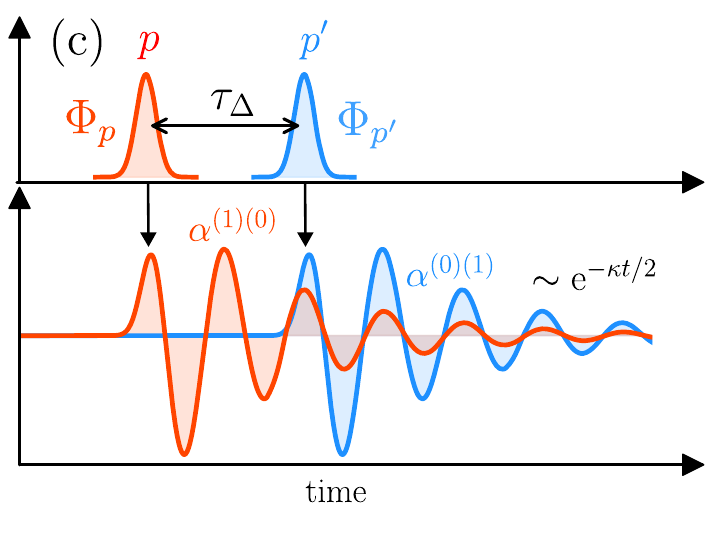
\includegraphics[width=\linewidth,height=0.55\textheight,keepaspectratio]
          {figures/prl_fig1c_pulse.png}\par}
      {\centering\fontsize{6.5}{7.6}\selectfont\color{gray}
        时间结构：$\tau_\Delta=\tau_{p'}-\tau_p$。由于腔内场具有有限寿命，某些微扰作用次序中 probe 场甚至可以先于 pump 场作用于分子体系。\par}
    \end{column}
  \end{columns}

  \vspace{0.8em}

  {\centering
    $\text{长延迟}\quad\Longrightarrow\quad
      \text{体系已接近稳/准稳状态，可近似使用 }\chi(\omega).$\\[0.2em]
    $\text{超短延迟？}$\\[0.2em]
    \par}

  \papersource{Reitz, Koner \& Yuen-Zhou,
    PRL 134, 193803 (2025), Fig.~1(a,c).}

\end{frame}
\begin{frame}{$N\to\infty$ 极限：腔场与单分子态自洽反馈}

  \footnotesize
  \setlength{\abovedisplayskip}{2pt}
  \setlength{\belowdisplayskip}{2pt}

  \[
    \begin{aligned}
      H_{\mathrm{MF}}(t)
        &=H_0+E_0[\alpha(t)+\alpha^*(t)]\hat\mu,\\[-1.5pt]
        \\
      \dot\rho
        &=-\ii[H_{\mathrm{MF}}(t),\rho]+\mathcal D[\rho].
    \end{aligned}
  \]

  \vspace{4em}

  \[
    \begin{aligned}
      \dot\alpha
        &=\physmark{Plum}{mfFree}{-\left(\tfrac{\kappa}{2}+\ii\omega_c\right)\alpha}
          \physmark{NavyBlue}{mfFeedback}{-\ii NE_0P}
          \physmark{OliveGreen}{mfInput}{-\eta f(t)e^{-\ii\omega_l t}},\qquad P&=\Tr[\hat\mu\rho].
    \end{aligned}
  \]
  \begin{tikzpicture}[overlay,remember picture,>=stealth,
      nodes={align=center,inner sep=1pt,font=\scriptsize},<-]
    \path (mfFree.north) ++(-1.5,1.0em)
      node[anchor=south,color=Plum] (mfFreeText)
      {腔模自由演化 + 振幅损耗};
    \draw[Plum] (mfFree.north) |- (mfFreeText.south);
    \path (mfFeedback.north) ++(0,1.0em)
      node[anchor=south,color=NavyBlue] (mfFeedbackText)
      {分子系综极化反馈};
    \draw[NavyBlue] (mfFeedback.north) -- (mfFeedbackText.south);
    \path (mfInput.north) ++(0.7,1.0em)
      node[anchor=south,color=OliveGreen] (mfInputText)
      {外部输入场驱动};
    \draw[OliveGreen] (mfInput.north) |- (mfInputText.south);
  \end{tikzpicture}

  \vspace{1em}
  {\centering
    \begin{tikzpicture}[>=stealth,thick,
        every node/.style={align=center,inner sep=3pt,font=\scriptsize}]
      \node[draw=Plum] (a) at (0,0)
        {$\alpha=\langle\hat a\rangle$\\腔内平均场};
      \node[draw] (h) at (3,0) {$H_{\mathrm{MF}}$\\驱动单分子};
      \node[draw] (r) at (6,0) {$\rho$\\分子量子态};
      \node[draw=NavyBlue] (p) at (9,0) {$P$\\单分子平均偶极};
      \draw[->] (a) -- (h);
      \draw[->] (h) -- (r);
      \draw[->] (r) -- (p);
      \draw[->,NavyBlue] (p.south) -- (9,-0.7)
        -- (0,-0.7) -- (a.south);
      \node[fill=white,text=NavyBlue] at (4.5,-0.7)
        {系综反馈：$NP$};
    \end{tikzpicture}\par}

  \papersource{Reitz, Koner \& Yuen-Zhou, PRL 134, 193803 (2025), Eqs.~(2)--(3).}

\end{frame}
\begin{frame}{腔内场与分子态的微扰展开}

  \footnotesize
  \setlength{\abovedisplayskip}{1pt}
  \setlength{\belowdisplayskip}{1pt}

  \[
    \alpha(t)=\sum_n\eta^n\alpha^{(n)}(t),
    \qquad
    \rho(t)=\sum_n\eta^n\rho^{(n)}(t).
  \]

  \vspace{0.3em}

  \begin{columns}[c,onlytextwidth]
    \begin{column}{0.48\textwidth}
      {\centering
        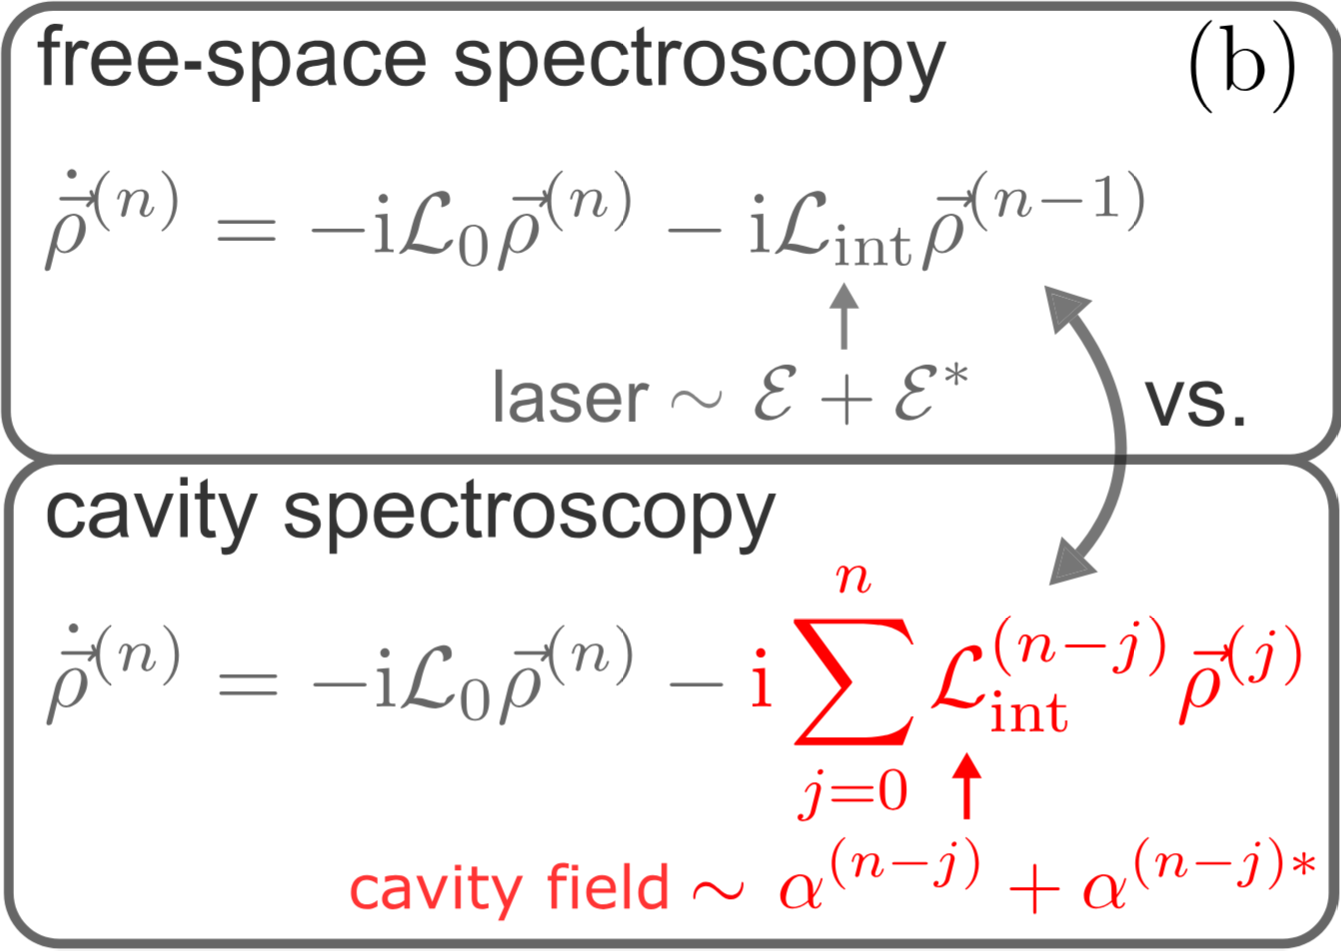
\includegraphics[width=\linewidth,keepaspectratio]{fig/fig1b.png}\par}
    \end{column}
    \begin{column}{0.50\textwidth}
      \scriptsize
      \[
        \dot\alpha^{(n)}
        =-\left(\tfrac{\kappa}{2}+\ii\omega_c\right)\alpha^{(n)}
        -\ii NE_0P^{(n)}
        -\physmark{OliveGreen}{ordDrive}{\delta_{n1}}
          f(t)e^{-\ii\omega_l t}.
      \]
      \begin{tikzpicture}[overlay,remember picture,>=stealth,
          nodes={align=center,inner sep=1pt,font=\scriptsize},<-]
        \path (ordDrive.south) ++(0.9,3.5em)
          node[anchor=north,color=OliveGreen,text width=3.0cm] (ordDriveText)
          {外部输入只驱动一阶};
        \draw[OliveGreen] (ordDrive.north) |- (ordDriveText.south);
      \end{tikzpicture}

      \vspace{3.5em}
      $n>1$ 的腔场由分子极化反馈产生。 

      自由空间：分子始终由给定的一阶激光场驱动；\\
      腔内：分子极化会产生新的高阶腔场。
  

    \end{column}
  \end{columns}

  \vspace{0.3em}

  \papersource{ PRL Fig.~1(b), p.~193803-2; Eqs.~(4)--(5).}
\end{frame}
\begin{frame}{腔反馈产生额外高阶演化路径}

  \footnotesize
  \setlength{\abovedisplayskip}{1pt}
  \setlength{\belowdisplayskip}{1pt}

  \[
    \physmark{NavyBlue}{p20tgt}{\dot{\vec\rho}^{(n)}}
    =\physmark{NavyBlue}{p20free}{-\ii\mathcal L_0\vec\rho^{(n)}}
    -\ii E_0\sum_{j=0}^{n}
    \physmark{Plum}{p20field}{
      \left[\alpha^{(n-j)}+\alpha^{(n-j)*}\right]}
    \mathcal L_\mu
    \physmark{Bittersweet}{p20rho}{\vec\rho^{(j)}}.
  \]
  \begin{tikzpicture}[overlay,remember picture,>=stealth,
      nodes={align=center,inner sep=1pt,font=\scriptsize},<-]
    \path (p20tgt.south) ++(-1.7,-1.1em)
      node[anchor=north,color=NavyBlue,text width=2.9cm] (p20tgtText)
      {目标：第 $n$ 阶分子响应};
    \draw[NavyBlue] (p20tgt.south) |- (p20tgtText.north);
    \path (p20free.south) ++(-0.3,-1.1em)
      node[anchor=north,color=NavyBlue!70!black,text width=2.6cm] (p20freeText)
      {自由演化，不产生新分支};
    \draw[NavyBlue!70!black] (p20free.south) -- (p20freeText.north);
    \path (p20field.south) ++(1.5,-1.1em)
      node[anchor=north,color=Plum,text width=2.2cm] (p20fieldText)
      {第 $n-j$ 阶腔场};
    \draw[Plum] (p20field.south) |- (p20fieldText.north);
    \path (p20rho.south) ++(2.6,-1.1em)
      node[anchor=north,color=Bittersweet,text width=2.6cm] (p20rhoText)
      {已有第 $j$ 阶分子响应};
    \draw[Bittersweet] (p20rho.south) |- (p20rhoText.north);
  \end{tikzpicture}
  \vspace{1.4em}

  \begin{columns}[c,onlytextwidth]
    \begin{column}{0.46\textwidth}
      {\centering
        \includegraphics[page=3,trim=321bp 565bp 57bp 47bp,clip,
          height=0.62\textheight,keepaspectratio]
          {../ref/Reitz 等 - 2025 - Nonlinear Semiclassical Spectroscopy of Ultrafast Molecular Polariton Dynamics.pdf}\par}
    \end{column}
    \begin{column}{0.52\textwidth}
      \scriptsize
      以二阶响应为例：
      \[
        \begin{aligned}
        \dot\rho^{(2)}
        &=-\ii\mathcal L_0\rho^{(2)}
          -\ii E_0\Big[
            (\alpha^{(1)}+\alpha^{(1)*})\mathcal L_\mu\rho^{(1)}\\
        &\qquad\quad
            +(\alpha^{(2)}+\alpha^{(2)*})\mathcal L_\mu\rho^{(0)}
          \Big].
        \end{aligned}
      \]
      {\color{gray}无外场时 $\alpha^{(0)}=0$。\par}
      \vspace{0.1em}
      {\centering\textcolor{orange!80!black}{%
        $\rho^{(0)}\xrightarrow{\alpha^{(1)}}
          \rho^{(1)}\xrightarrow{\alpha^{(1)}}\rho^{(2)}$}\par}
      \textcolor{orange!80!black}{连续两次一阶作用：自由空间已有的路径。}
      \par\vspace{0.1em}
      {\centering$\rho^{(0)}\xrightarrow{\alpha^{(2)}}\rho^{(2)}$\par}
      $\alpha^{(2)}$ 由分子极化反馈产生。
      \par\vspace{0.1em}
    \end{column}
  \end{columns}

  \papersource{Reitz, Koner \& Yuen-Zhou, PRL 134, 193803 (2025), Eq.~(5b), Fig.~2.}

\end{frame}
